\chapter {MOTION SYNTHESIS FRAMEWORK}
\label{chap:msf}
\nomenclature[z57]{\boa}{Basin of Attraction}
\graphicspath{{CombineFramework/CombineFrameworkFigs/EPS/}{CombineFramework/CombineFrameworkFigs/}}
The principal ideas of \moit are discussed in previous two chapters.
Stability of motion is controlled by maintaining the topology, 
for periodic motion, neural oscillator can be used to enhance the structural stability.
And group Transformation provides a mechanism to modify motion with precision.


Questions rise when these ideas are being applied  to \cms.
The first question comes from combining the controller of neural oscillator and symmetry controller.
We must ensure that the combination will violate neither the symmetry nor the topology,
This question is discussed in details in Section~\ref{sec:combin}.


Section~\ref{sec:procframe} provides more detailed information of the pipeline, or the procedure of applying this idea in \cms applications

%Previous chapters only focus on how to maintain motion primitives, a further question is how motion primitives are connected, for example, how a character transit from walking to running. 
%Section~\ref{sec:manyprimitive} shows how the method for maintaining motion primitive are used for motion primitive transition.
%
%
%
%
%The ideas of Global Motor Invariant and Local Motor Invariant are discussed separately in Chapter~\ref{chap:gi} and Chapter~\ref{chap:li}.
%This chapter focuses on put these ideas into \cms application.
%Two problems arised from combinations in application
%\begin{itemize}
%	\item Combine global and local motor invariant controller together.
%	\item Combine different motion primitives together.
%\end{itemize}

\section{Combined Invariant Control}
\label{sec:combin}
\subsection{ Combine Invariant Control}

Neural control $\uout$ will maintain the topology and local control $ulocal$  maintains the symmetry.
Combining two controllers will violate nor the global or local invariant:
From the perspective in Chapter~\ref{chap:gi},
when the controlled symmetry  is applied, it must not violate the topology. 
It is easy to prove that controlled symmetry maintains the topology.
For the controlled symmetry's effect on topology, we have the following theorem:

\begin{mythe}
Transformation of Control Symmetry is Topological Conjugation
\end{mythe}


From the perspective in Chapter~\ref{chap:li},
we must ensure the inclusion of neural oscillator control $\ulocal$ will not break the controlled symmetry.


In application, to adjust the combined controller,
\cpg is applied first to maintain the topology against the structural perturbation. 
Afterwards Symmetry Control is to meet application specific constraints.
This idea is illustrated in the following Figure ~\ref{fig:sysoverview}

\begin{figure}[!htbp]
  \begin{center}
      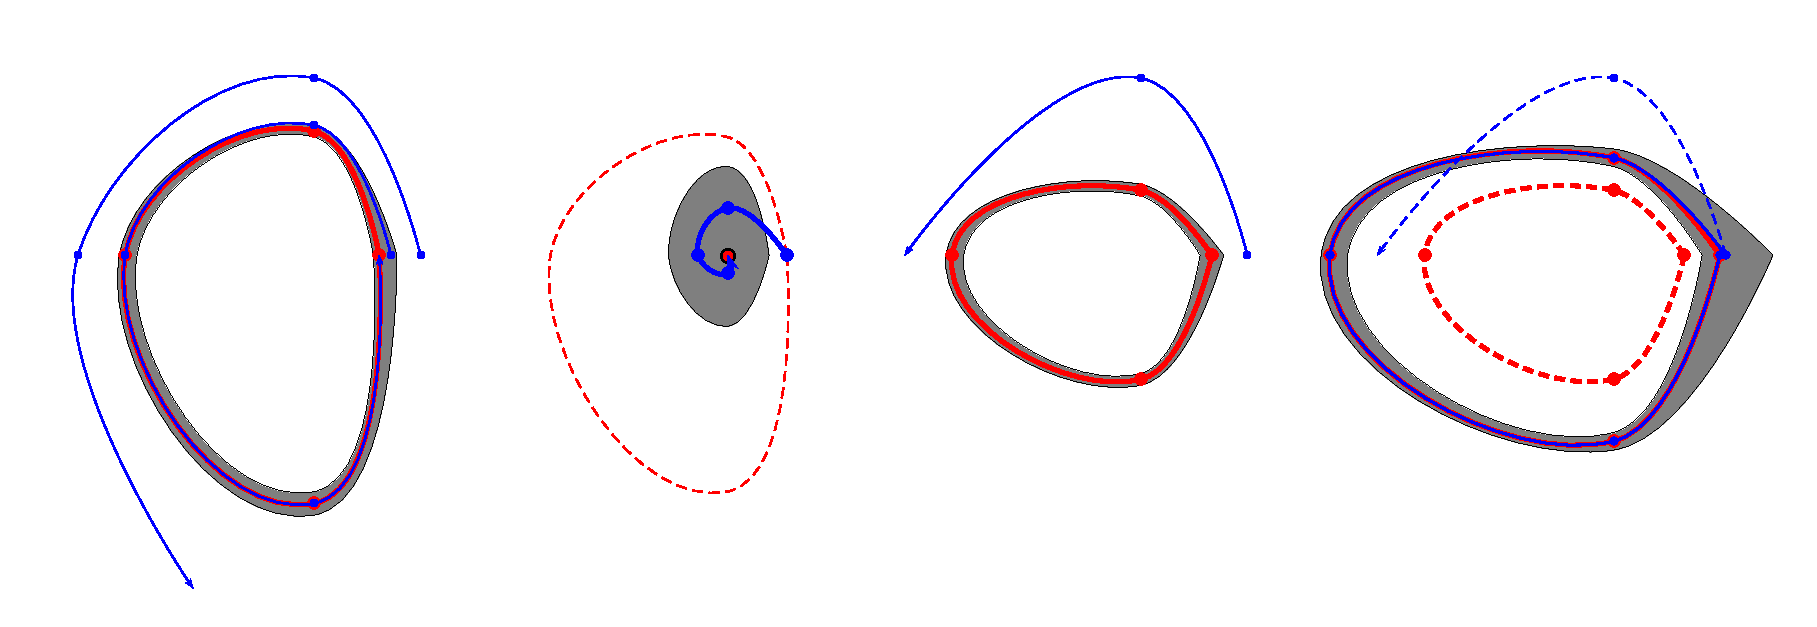
\includegraphics[width=0.7\textwidth]{LimitCircle}
    \caption{System Over View }
    \label{fig:sysoverview}
  \end{center}
\end{figure}

When a group action is applied to the mechanical system, parameters of \cpg should be transformed accordingly to maintain the symmetry property.
This is called \emph{Adjoint Transformation}.









\subsection{Adjoint Transformation of \cpg}
\emph{Adjoint Transformation} modifies the parameters of neural oscillator to maintain the symmetry.

For a dynamic system 
\[
\dot{\state}=F(\state)
\]
when controlled by neural oscillator, it becomes 
\begin{equation}
\label{eq:gc}
\dot{\state}=F(\state)+D\uout
\end{equation}
where $D$ is the connection matrix, which describes how the neural oscillator is connected to mechanical system.


When group action $g$ is applied, the Equations~\ref{eq:gc} is transformed into
\begin{equation}
\label{eq:cc}
Tg(\dot{\state})=F(g(\state))+DTg(\uout)
\end{equation}




If symmetry is preserved, the Equation~\ref{eq:con} and Equation~\ref{eq:cc} should be equivalent.
\begin{equation}
\label{eq:con}
\dot{\state}=F(\state)+\ulocal+D\tilde{\uout}
\end{equation}
where $\tilde{\uout}$ is the output of neural system after adjoint transformation.

As shown in Equation~\ref{eq:simplematsuta},$\uout$ is a complex function of $\uin$.
Developing close form formula will be difficult and not computational efficient.
By exploring the symmetry property of Matsuoka Oscillator, transformation can be achieved by modifying the parameters.
we have the following proposition.


\begin{myprop}
By modifying parameter $\tau_{1,2}$
\[
\tau_{1,2} \mapsto \ep \tau_{1,2}
\]
is equivalent to time scaling the neural oscillator by parameter $\ep$.
\end{myprop}

This proposition can be easily proved by  substituting $\tilde{\tau}_{1,2}=\ep \tau_{1,2}$, and $\tilde{t}=\frac{t}{\ep}$ into the Matsuoka Oscillator( Equation~\ref{eq:matsuta}), the equation will remain the same.
Based on the proposition above, a scheme of adjoint transformation to modify the parameters $\tau_{1,2}$,$\hin$,$\hout$ for maintain the symmetry of the  coupled system.
The input and output of neural are chosen to maintain the shape.
\begin{enumerate}
\item Modify $\tau$ by the time scaling parameter $\tau \mapsto \ep \tau$.
\item Input variable $w$ and input efficient $\hin$ are modified to make sure the input function satisfy the time scaling symmetry $\uin(t) \mapsto \uin(\frac{t}{\ep})$
\item  Parameters of $\hout$ are modified according to connection matrix $D$, or how the mechanical system is drived.
If $\uout$ drives the position variable $q$ then, $\hout$ should multiplied by the position scale factor. 
If $\uout$ drives the velocity,$\hout$ is multiplied by the speed scale factor.
If the $hout$ is force and acting on the acceleration $\ddot{q}$, then $\hout$ is multiplied by the acceleration scale factor.
\end{enumerate}


According to this adjoint transformation strategy, we can get the following theorem
\begin{mythe}
For a transformation group $G$, if the parameters of the neural oscillator are modified according to adjoint transformation,
combined system preserves symmetry $I^G$.
\end{mythe}
For proof, readers can check the symmetry by substituting transformed variables into the original system to check the symmetry.
Thus both the Local Motor Invariant and Global Motor Invariant are maintained
For the specific symmetry types proposed in Chapter~\ref{chap:li},several examples of adjoint transformations are provided


\subsubsection*{ Offset Symmetry.}
For offset symmetry:
\[
(t,q,\qd) \mapsto (t,q+\ep,\qd)
\]
there is no time scaling effects.
To maintain the symmetry,  the simplest way is to select $\uin$ and $\uout$ from functions from invariant space$I^G$.
For example, when all the $q$ is transformed by a constant, the difference and the velocity will not be transformed. 
Thus,the input of the neural oscillator is chosen to be the angle difference between the joints or velocity.



\subsubsection*{Time Scaling}
For time scaling:
\[
(t,q,\qd) \mapsto (\frac{t}{\ep},q,\ep \qd)
\]
Adjoint Transformation
$\tau \mapsto \ep \tau $.
The input coefficient $\hin$ and output coefficient $\hout$ are scaled accordingly.
if the output$\uout$ is applied as force, then it should be scaled by the acceleration factor
\[
 \hout \mapsto \ep^2 \hout
\]
\subsubsection*{ Energy Scaling}
Energy Scaling is combined action of time scaling and posture scaling:
\[
(t,q,\qd ) \mapsto ( \frac{f(\ep)}{\ep}t ,f(\ep)q,\ep\qd)
\]
the time scaling factor is $\frac{\ep}{f(\ep)}$, 

The parameters $\tau_{1,2}$ are transformed
\[
\tau_{1,2} \mapsto \frac{\ep}{f(\ep)} \tau_{1,2}
\]

The input coefficient is scaled to make the amplitude of the input signal maintained.
\[
\hin \mapsto \frac{\hin}{\ep}
\]

The output coefficient is scaled according to the connection of the control, 
if the output is drive the velocity, then the output is $\hout$
\[
\hout \mapsto \ep \hout
\]




\subsection{Example: Height Control of Bouncing Ball}

The Bouncing Ball has the energy scaling symmetry; a limit cycle emerged when coupled with neural oscillator.
By combining both motor invariant controllers, energy transformation can be applied to the limit cycle.
and the ball  bounces about a constant height with robust stability.

\subsubsection*{Adjoint Transformation}
Supposing the coupled system is bouncing at height of $5$
For the energy scaling:
\[
(t,q,\qd ) \mapsto ( \ep t ,\ep^2 q,\ep \qd)
\]
and he time scaling factor is $\ep$, we have:
\[
\tau_{1,2} \mapsto \ep \tau_{1,2}
\]

The input to the neural oscillator is $\qd$,
\[
\hin \mapsto \frac{\hin}{\ep}
\]
 
Neural Oscillator drives the position of the paddle, the output $\uout$ needs to be scaled by the position scale value.
For $q \mapsto \ep^2q$, we have
\[
 \hout \mapsto \ep^2 \hout
\]

When $\ep^2=3$,  the ball will bounce at height of $15$, and it maintains its topological structure, which is a limit cycle, as shown in Figure ~\ref{fig:energy3}. 
With this method, arbitrary bouncing height can be controlled.


\begin{figure}[!htbp]
  \begin{center}
   	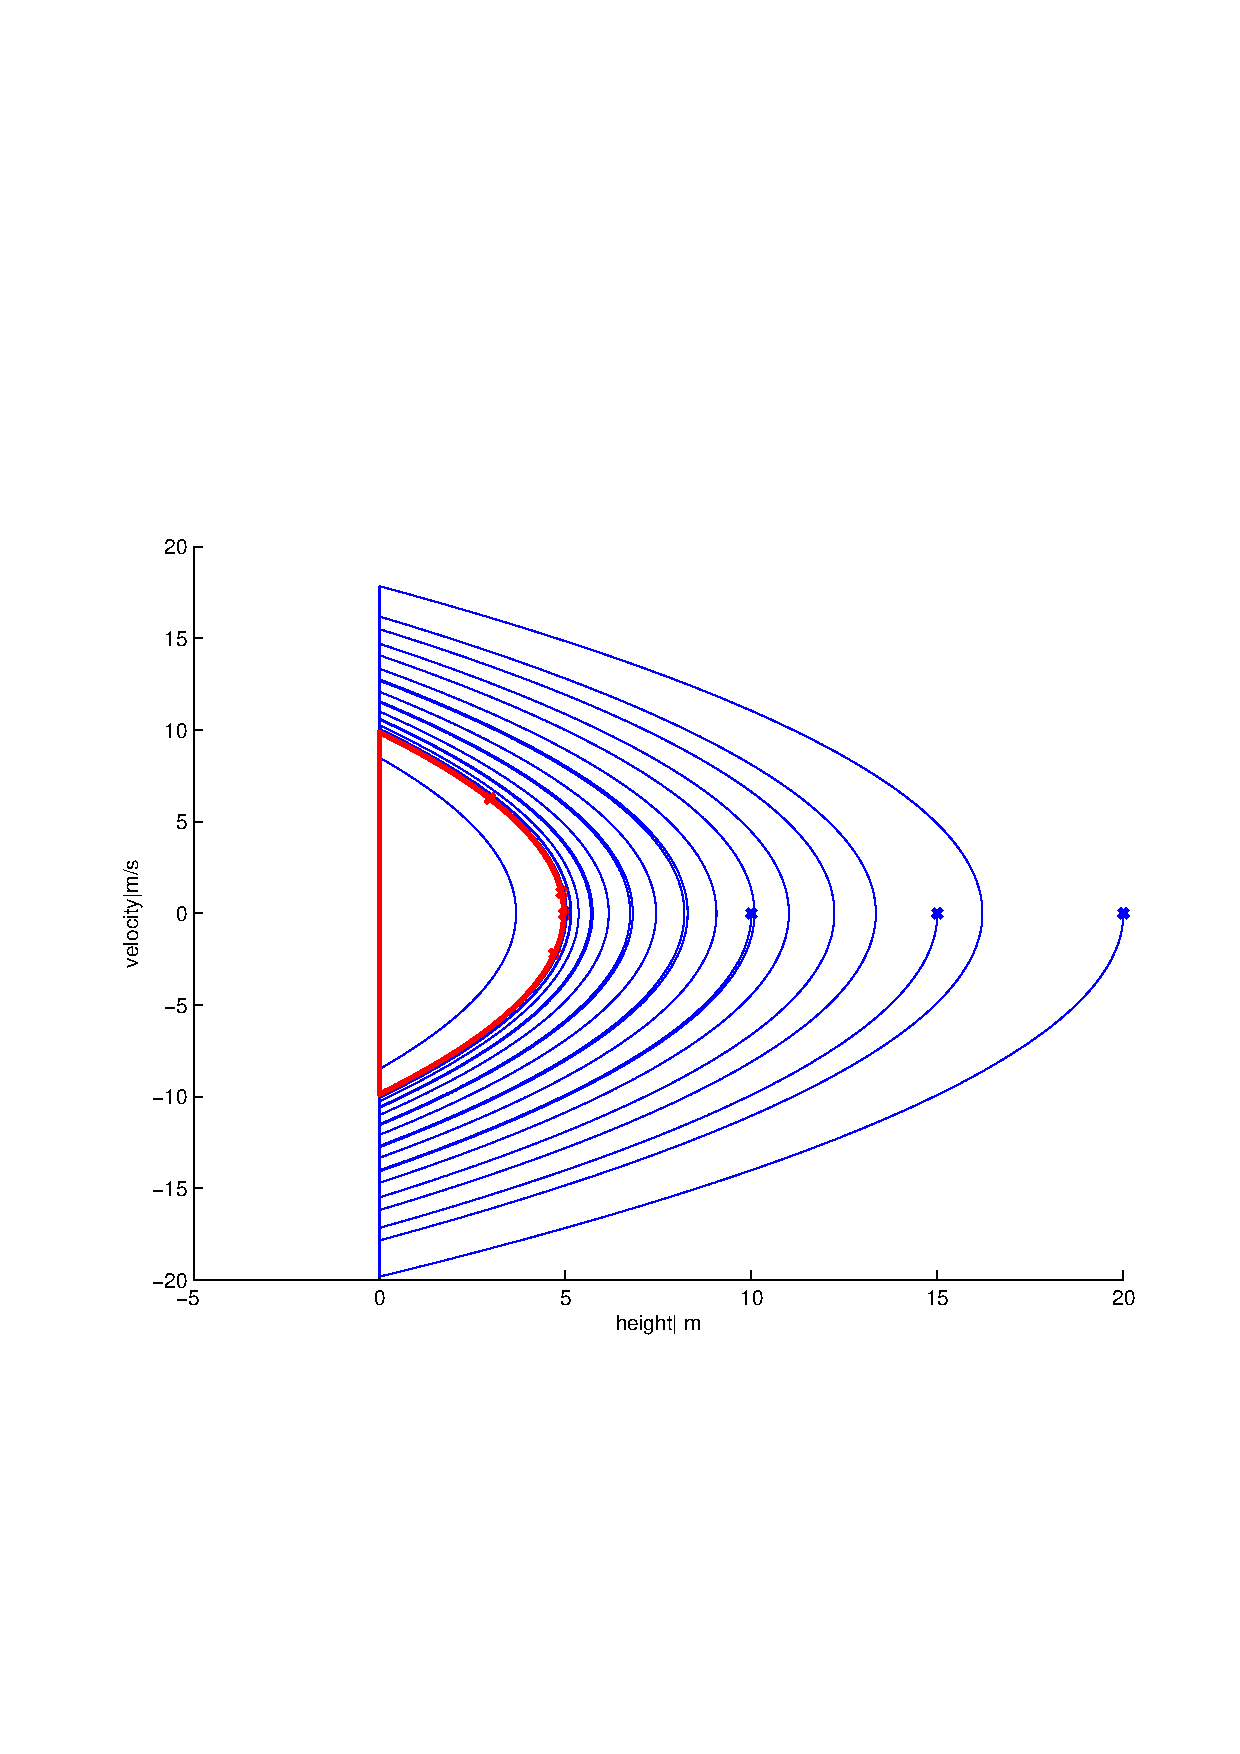
\includegraphics[width=0.7\textwidth]{BouncingBallPhasePlotAction1}
    \caption{Energy Scalling}
    \label{fig:energy1}
  \end{center}
\end{figure} 


\begin{figure}[!htbp]
  \begin{center}
	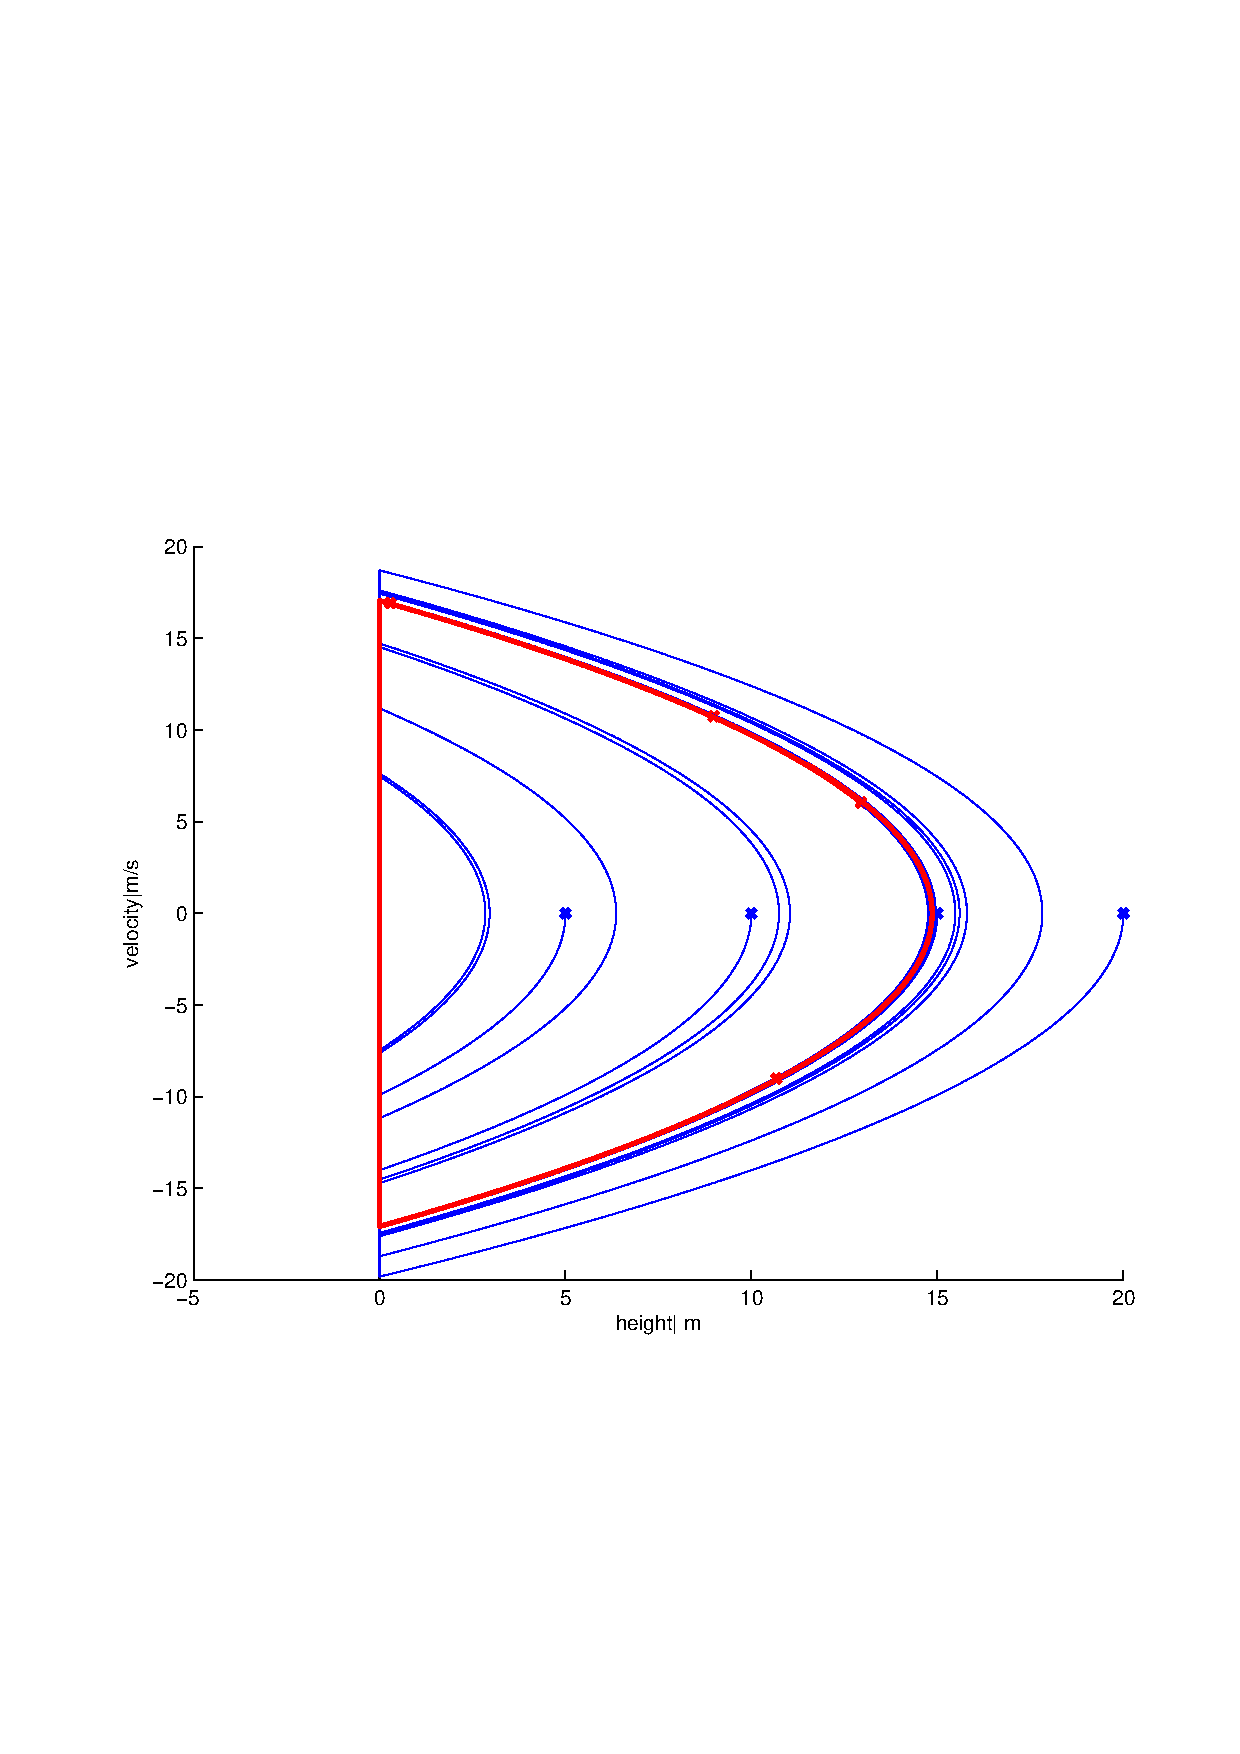
\includegraphics[width=0.7\textwidth]{BouncingBallPhasePlotAction3}
    \caption{Energy Scaling}
    \label{fig:energy3}
  \end{center}
\end{figure}

\section{Combine Motion Primitives}
\label{sec:manyprimitive}

\subsection{Dynamic Motion Graph}
Virtual characters are capable of many type of motions and change its motion fluently.
\emph{Motion Graph}\citep{kovar2008motion} is proposed for data-driven \cms:
basic motion tasks are recorded, and a graph describes how a character can change from one motion into another motion. 
The most popular method for synthesizing transition motion is through motion blending.


\moit reaches a similar idea to motion graph through a different direction.
Usually, traditional \emph{motion graph}s are manually designed, \moit proposes the idea generating the motion graph from the dynamics.
In theory,the topological structure of a dynamic system can be represented by a  graph.
Each motion primitive is represented as a node, and two nodes are connected only if their basin of attraction(\boa)s are in neighbour.

\begin{figure}[!htbp]
  \begin{center}
	\includegraphics[width=0.7\textwidth]{MotionPrimitiveGraph}
    \caption{Phase Plot of Motion Primitives}
    \label{fig:manyprimitives}
  \end{center}
\end{figure}


\begin{figure}[!htbp]
  \begin{center}
      \includegraphics[width=0.7\textwidth]{motiongraphtopology}
    \caption{The Graph Structure of A Dynamic System}
    \label{fig:manyprimitivesgraph}
  \end{center}
\end{figure}

For example, Figure~\ref{fig:manyprimitives} shows the phase portrait of a hypothetical dynamic system,its phase space is divided into four region in different color, the four \boa s, within each region, there is a limit cycle(deep coloured).
The graph in Figure~\ref{fig:manyprimitivesgraph} shows the corresponding graph structure, in which each node represents the \boa of the same color in Figure~\ref{fig:manyprimitives}, the connecting edge means the basin of {\boa}s of connected motion primitives are in neighbour, which can also be verified in Figure~\ref{fig:manyprimitives}.


\subsection{Dynamic Motion Transition}
The transition of motion plays a very important role in \cms.
Blending techniques tend to generate motions with little variation, while in reality, many variations happen during transition.
\moit introduces the physics based method for generation of transition motion, which is exactly based on the control method for maintaining motion primitives.


\begin{figure}[!htbp]
  \begin{center}
      \includegraphics[width=0.7\textwidth]{MotionPrimitiveTransition}
    \caption{Motion Primitive Transition}
    \label{fig:motion-transition}
  \end{center}
\end{figure}

From  geometrical perspective, motion transition means transform $\state$ from one \boa into another.
As shown in Figure~\ref{fig:motion-transition}, the current state represented by the black dot lies in the left region of \boa, over the time, it will converge to the red limit cycle.

The neighbouring region is the \boa of another primitive, in which if the current state lies, will converge to the green limit cycle.
Without any effort, the transition will not happen automatically, for the two basic of attractions do not overlap.
Motion Transition only needs a small action to push the state across the boundary, represented by the red line.
This idea implies many efficient method.


\subsubsection*{Entrainment Overlap}
Empirically,when \cpg is applied for one motor primitive $\mathcal{A}$, the \boa $\BOA{A}$ is enlarged.
Supposing the enlarged \boa  is  represented by $\BOA{A'}$.
If \cpg are applied for two motion primitives $\mathcal{A_1,A_2}$ separately, the enlarged basin of attractions are $\BOA{A_1'}$ and
%$\omicron$
$\BOA{A_2'}$ will overlap. 
Supposing the overlap region is $O$,
then we have
\[
O =
\BOA{A_1'} 
\bigcap \BOA{A_2'} 
\neq \varnothing
\]

\begin{figure}[!htbp]
  \begin{center}
      \includegraphics[width=0.7\textwidth]{OverLayTransition}
    \caption{OverLay Transition}
    \label{fig:motion-overlay}
  \end{center}
\end{figure}
 
If  state $\state$ lies in the $O$, by switching the \cpg controller, motion primitive is also switched.
Figure~\ref{fig:motion-overlay} shows the idea through an example, one the phase plot shown two motion primitives which are connected.
Basin of attractions of natural dynamics are represented by the dot line, \boa of natural dynamics are not overlay.
When \cpg is applied, two \boa are enlarged, and the shared region are coloured in pink color.
When the current state lies in $O$, if the \cpg of the left region is activated, the state will converge to the left limit cycle,
if the right \cpg is activated, the state will converge to the right limit cycle.
Motion Primitive can be switched in this manner.






\subsubsection*{Transform Method}
Controlled Symmetry can also apply for motion primitive transition.
We can change the \boa in which the current state lies by transforming the phase portrait.

\begin{figure}[!htbp]
  \begin{center}
      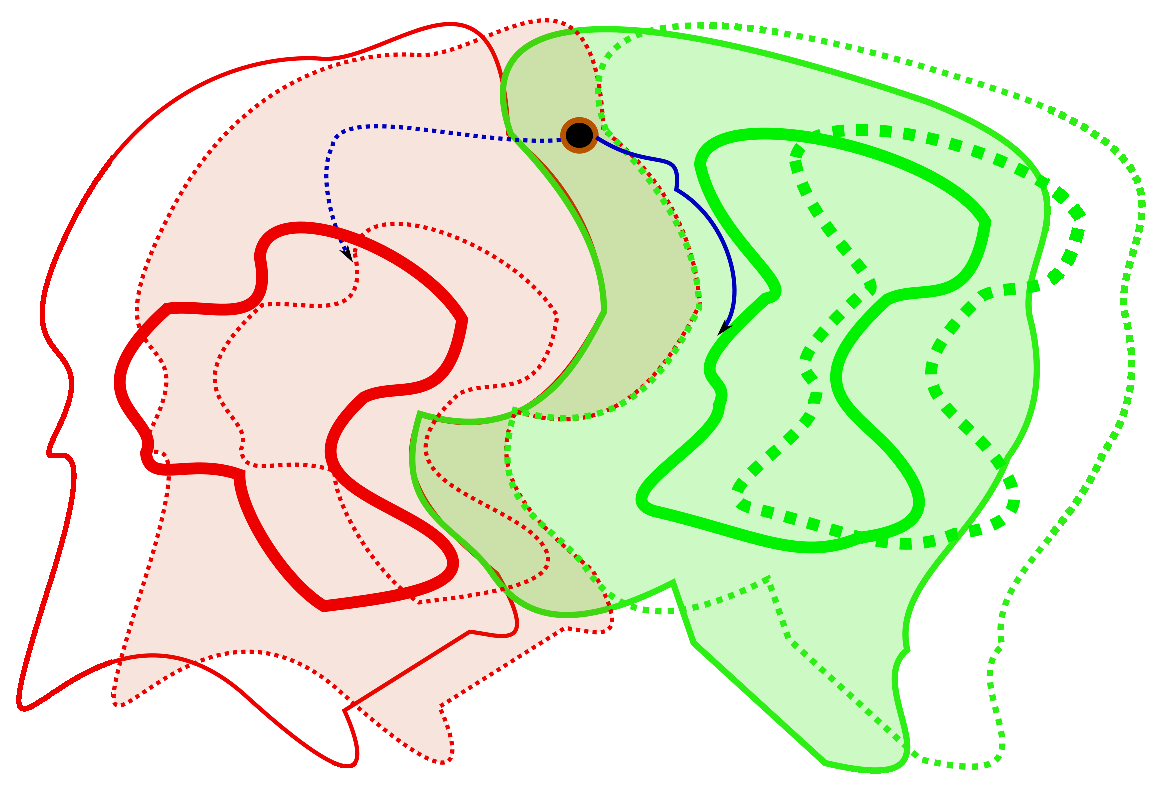
\includegraphics[width=0.7\textwidth]{OffsetTransition}
    \caption{Offset Transition}
    \label{fig:transform-offset}
  \end{center}
\end{figure}




As shown in Figure~\ref{fig:transform-offset}, the phase portrait of natural dynamic system is the same as that of Figure~\ref{fig:motion-overlay}, which is also drawn by the dot.
The current state converges to the left (red) limit cycle.
By applying offset action to the dynamic system, the phase portrait  moves leftward, which make current state lie in the right \boa.
Over the time, current state will converge to the right(green) limit cycle, accordingly, motion primitive is changed.







\subsection{Combined Method}
Both methods utilize the natural dynamics and  result in physically realistic transition.
The passivity also permits variability but requires $\state$ lies at specific region.
In motor invariant theory, the current state $\state$ is not directly controlled,
The measure taken is to make the overlap region $O$ cover part of both attractors.

As shown in Figure~\ref{fig:Combine}
The overlap region covers both attractors $\mathcal{A}$, $\mathcal{A'}$,bidirectional transitions are possible when motions are near stable state.

More importantly, when transformation is applied, both motion primitives are transformed, this is the \emph{connection transformation }. 
As shown in Figure~\ref{fig:Combine}, both motion primitives are transformed by the time scaling action.

\begin{figure}[!htbp]
  \begin{center}
      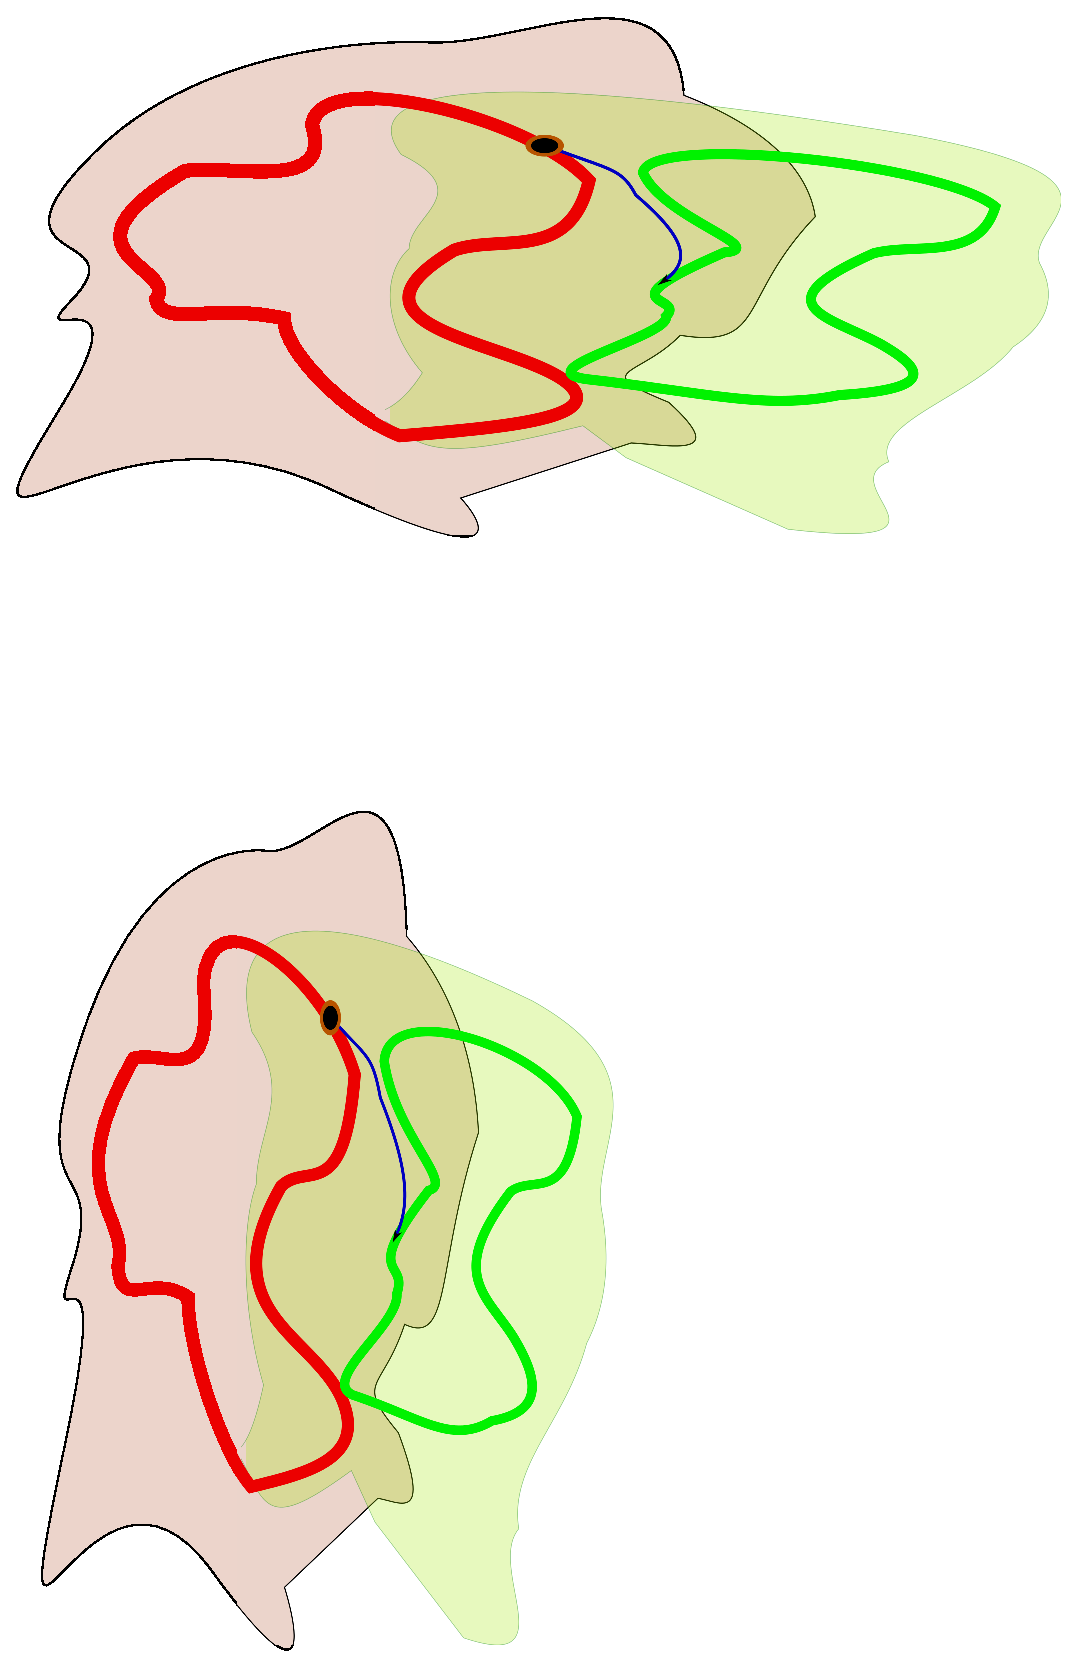
\includegraphics[width=0.7\textwidth]{ConbineMethod}
    \caption{Combined Method}
    \label{fig:Combine}
  \end{center}
\end{figure}

\section{Motion Synthesis Framework}
\label{sec:procframe}
While this procedure may appear mathematically complex, applying this method for motion synthesis is straightforward. 
You will need:
\begin{enumerate}
\item a mechanical oscillator $F(\x)$ which best describes the body and environment
\item a neural oscillator (for example, the Matsuoka oscillator in Equation~\ref{eq:matsuta}) and associated parameters,that form a limit cycle

\item an action $g \in G$ which adapts the problem to the current environment (we present three possible operators in Section~\ref{sec:groupandsymmetry}). 
The adjoint system transformation  is applied to the neural oscillator parameters.

\item an integrator to solve the system (we use the fourth order Runge--Kutta method provided in the {MATLAB} function \emph{ode45}).
\end{enumerate}
In the following chapters, this method is applied to generating adaptive motions.



